  A torre de sustentação da turbina tem como função suportar todo o peso do rotor e da nacele e erguer este conjunto a uma altura onde as pás possam girar com segurança e distantes do solo. A altura da torre tem uma relação direta com a capacidade de produção de energia, sendo que quanto mais alto a torre for, maior será essa produção devido ao maior fluxo de vento. Com os ventos constantes, o que determinará a quantidade de energia a ser gerada é o diâmetro do rotor. O diâmetro do rotor da turbina tratada neste projeto é de 18,5 m, possuindo um torque médio em seu eixo de   4775, 5 N.m e com a necessidade de gerar 50 kW. A seguir uma breve relação entre o diâmetro do motor e a geração máxima de energia capaz de ser produzida por uma turbina eólica tradicional. \footnotemark
  \footnotetext{<http://www.fiec.org.br/artigos/energia/energia\_eolica.htm>. Acesso em 26 maio de 2015.}
  
  \begin{figure}[!h]
    \centering
    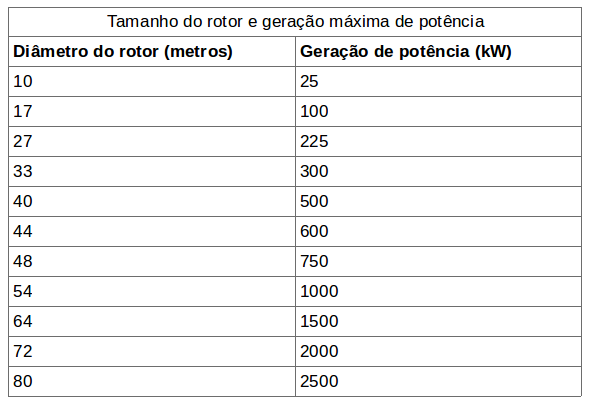
\includegraphics[scale = 0.5]{editaveis/figuras/tamanho_rotor}
    \label{tamanho_rotor}
    \caption[Tamanho do rotor e geração máxima de potência]{Tamanho do rotor e geração máxima de potência. \footnotemark}
   \end{figure}
   \FloatBarrier
   \footnotetext{Fonte: Associação Dinamarquesa da Indústria Eólica, Associação Americana de Energia Eólica.}
   
   Existem três tipos de torre utilizadas para a afinidade buscada: a tubular em aço, a tubular em concreto e a treliçada e quanto ao porte: pequeno, intermediário e grande porte. A turbina do projeto foi enquadrada como porte intermediário (10 - 250kW).  Devido ao aumento do peso dos componentes suportados pela nacele e das próprias pás ao longo dos anos, tem-se usado atualmente as torres tubulares de metais ou de concreto para assegurar a sustentação e suportar tensões provocadas por altitudes cada vez mais altas \footnotemark. Por este motivo e pela elevada preferência pelo mercado nesse tipo de torre, foi escolhido a torre tubular.
   \footnotetext{Disponível em: <http://www.cresesb.cepel.br/download/tutorial/tutorial\_eolica\_2008\_e-book.pdf>. Acesso em: 26 mai. 2015.}
   
   As torres cônicas tubulares podem ser compostos por aço, material relativamente barato e de montagem rápida podendo ser realizada no próprio lugar de instalação; Betão, que pode ser tanto construída no local como pré-moldado, porém é menos flexível que as torres de aço, ou podem ser híbridas, onde sua base é construída de concreto  e seu corpo principal de aço (As torres são frequentemente acoplada com parafusos às concretas bases sobre as quais repousam). \footnotemark
   \footnotetext{Fonte: Energias Renováveis: Energia Eólica 26/06/2014 Por : Luís Timóteo 3.}
   
   Depois de semanas de pesquisas, cruze de dados e comparações entre diversos modelos de torre, a equipe da frente de mecânica optou por utilizar uma torre de aço Q415 que passa por um processo de galvanização quente e pintado com spray, dando a capacidade de proteger a torre contra corrosão e ferrugem. \footnotemark
   \footnotetext{Disponível em: <http://www.chinahummer.cn/index.php/index/content/45>. Acesso em: 19 mai. 2015.}
   
   Partindo do princípio que a velocidade do vento necessária para a produção de energia desejada é a mínima do local de instalação das turbinas, definimos a altura como uma distância segura do solo apenas, tendo em vista que não precisamos colocar o rotor a uma determina altitude para que alcance uma determinada velocidade do vento. Desta forma, escolhemos uma torre com as seguintes especificações: 
   
   \begin{figure}[!h]
    \centering
    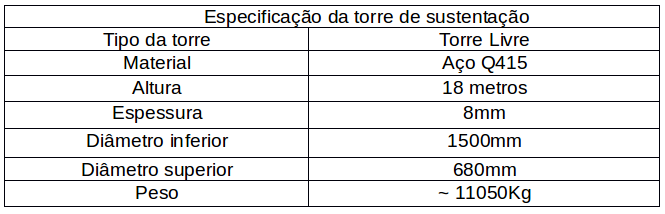
\includegraphics[scale = 0.5]{editaveis/figuras/torre_spec}
    \label{torre_spec}
    \caption[Especificação da torre de sustentação]{Especificação da torre de sustentação. \footnotemark}
   \end{figure}
   \FloatBarrier
   \footnotetext{Disponível em :< http://1047121.en.makepolo.com/products/50KW-Wind-Turbine-Generator-p41716180.html>. Acesso em 20 mai. 2015.}
   
   Quanto ao material utilizado nessa torre, trata-se de um Aço Inox 415. O aço inoxidável pertence à classe Martensítica e possui uma adição de elementos em sua composição química que aumenta a resistência à corrosão em relação aos martensíticos tradicionais. Comparado com os aços 410 e 420, o aço 415 contém uma quantidade menor de carbono, o que confere um diferencial para esta liga. Esta liga passa por um processo de têmpera para  que suas propriedades mecânicas e de dureza se elevem, posteriormente passando também por um processo de revenimento para aliviar as tensões internas do material provocadas pela têmpera. Sua aplicação é importante em ambientes onde o material está exposto a atrito, corrosão e abrasão, devido a estes fatores, a aplicação desta liga na construção de torres de sustentação para turbinas eólicas são constantes.\footnotemark
   \footnotetext{Disponível em:< http://www.megaligas.com.br/produtos\_aco\_inox\_S41500.asp>. Acesso em: 20 mai. 2015.}
   